%
% CS 109b Final Project 
%

\documentclass{article}
\usepackage[margin=1in]{geometry} % margins
\usepackage{amsmath} % math symbols
\renewcommand{\baselinestretch}{1} % line spacing
\usepackage{graphicx} % images
\graphicspath{ {images/} } % image directory
\setlength\parindent{0pt} % no indent
\usepackage{subfig}
\usepackage{lipsum}
\setlength\parindent{16pt}

% Floor and Ceiling Functions
\newcommand\floor[1]{\lfloor#1\rfloor}
\newcommand\ceil[1]{\lceil#1\rceil} 

% URL stuff
\usepackage{hyperref}
\hypersetup{
    colorlinks=true,
    linkcolor=blue,
    filecolor=magenta,      
    urlcolor=cyan,
}
 
\urlstyle{same}

% Headers & Footers 
\usepackage{fancyhdr}
\usepackage{lastpage} % allows for Page X of Y
\pagestyle{fancy}
\fancyhf{}
\lhead{CS 109b: Advanced Topics in Data Science}
\rhead{Final Project: Predicting Movie Genres}
\cfoot{Page \thepage \hspace{1pt} of 6}

\begin{document}

\thispagestyle{empty} % suppresses headers on first page

\begin{center}
    \LARGE{CS 109b Final Project} \\
    \smallskip
    \normalsize{Project Group 6} \\
    \normalsize{Christopher Chen, Phillip Huang, Harry Xue, Ted Zhu}
\end{center}

\section{Introduction}
\indent

In this project, we tackled the problem of predicting movie genres based on metadata and movie posters. In the first part of our project, we used aggregated data from multiple sources to train our models. From examining the data we obtained, we decided to conduct multilabel classification, using movie metadata for non-deep-learning models and using movie posters for deep learning models.

\section{Methods}
    \subsection{Data Collection}
        
        \indent
        
        \textbf{IMDb 5000:}
        For exploratory data analysis on the relationship between movie genres and movie metadata, we used the \href{https://www.kaggle.com/deepmatrix/imdb-5000-movie-dataset}{IMDb 5000} dataset because it was already cleaned and well-formatted. Since it contained only 5000 movies with no guarantees about genre frequencies, we did not use this dataset for any other tasks.
        
        \textbf{TMDb:}
        From researching multilabel classification methods, we knew that label imbalance in training data (extremely different numbers of movies in each genre) creates problems for multilabel classification algorithms. 
        To address this problem and acquire a relatively large number of data observations, we scraped metadata and posters for the 1,000 most popular movies in each genre using the \href{https://developers.themoviedb.org/3/discover}{Discover function} in the TMDb API for a total of approximately 11,000 unique movies.
        
        \textbf{IMDb:}
        To enrich the set of predictors in our data, we decided to scrape additional metadata from IMDb for each movie. We accomplished this by fetching the IMDb ID for each movie using the \href{https://developers.themoviedb.org/3/find}{\texttt{find} function} in the TMDb API then fetching the IMDb data by using IMDb IDs with the \href{http://imdbpy.sourceforge.net/}{IMDbPY module} for Python.
        
        \textbf{Label Imbalance Concerns:}
        The reason we only had 11,000 unique movies across 20 genres and could not guarantee absolutely equal distribution of labels (genres) in our dataset was due to the two ways that movies and genres co-occur: (1) The same movie appears across multiple sets of 1,000 movies for the different genres; (2) A movie sampled in one set of 1,000 movies for a given genre was not popular enough to appear in any other sets, but contains multiple genres. After calculating genre frequencies in our final metadata training set, we found that they were all approximately between 0.1 and 0.2, which we believed was an acceptable level of label imbalance.
        
        \textbf{Train/Test Split:}
        Before training our models, we split the data into 3 sets: 80\% train, 10\% validation, and 10\% test. We held out the test set until we were ready to evaluate our final best models (that were tuned on the validation set) to prevent any information leakage.
        
    \subsection{Traditional Machine Learning Methods for Classification}
        \indent 
        
        Predicting movie genres is a multi-label classification problem because each movie can have more than one genre. We utilized a variety of problem transformation methods and algorithm adaptation methods in tackling the multi-label problem, because each method used possessed unique advantages the others did not have. Each of these methods were fit on the metadata only. 
        
        \textbf{Algorithm Adaptation:}
        Used a random forest model as our direct application of an algorithm to a multi-label problem. This works because random forests can natively handle multi-label predictions with multilabel entropy.
        
        \textbf{Problem Transformation:}
        Problem transformation methods turn the multi-label problem into a single-label problem, and fit standard models on the transformed problem. We used the following models, chosen by their superior performance in prevailing academic literature and by their suitability to the movie dataset:
        
        \begin{itemize}
            \item Binary Relevance (BR): Ignores label dependency but simple and flexible. Also known as One v. All.
            \item Ensembles of Chained Classifiers (ECC): An ensemble of Chained Classifiers, which are a variation of BR that uses results from previous models as predictors for future models. This is a improvement because it allows for some modeling of label dependencies by greedily approximating them in a fashion similar to the ``chain rule'' from calculus. 
            \item Random k-Label Subsets (RAKEL): An improvement on the Label Powerset (LP) method. LP directly takes into account label dependencies by considering all possible sets of genres, but drastically increases model complexity by adding many features. RAKEL mitigates the complexity problem by taking only a small random sample of size $k$ of the sets for each model in the ensemble. It is conceptually very similar to random forests.
            \item Ensembles of Pruned Sets (EPS): An improvement on LP. Mitigates complexity problem by removing observations with rare sets of genres and replacing them with observations with sets of genres that are more popular. 
            \item Hierarchy of Multi-label Classifiers (HOMER): An improvement on LP that constructs a hierarchy of multi-label classifiers, with each one lower in the hierarchy dealing with a smaller set of labels.
        \end{itemize}
        
        We used random forests as the backend for all of the problem transformation problems due to their speed and generally high out-of-the-box performance. Each of the problem transformation methods were implemented in R using the \href{https://cran.r-project.org/web/packages/utiml/utiml.pdf}{\texttt{utiml}} library, as Python does not yet have a mature package that supports these fairly cutting-edge methods.  Each of the LP-based methods are well-suited to data sets with many labels, as is the case with our movie data set. We also briefly experimented with using the bottleneck features from VGG-16 in a random forest, but abandoned this approach after seeing poor results.
    
    \subsection{Deep Learning}
        \indent 
        
        \textbf{CNN from Scratch:} To build a simple convolutional neural network (CNN) from scratch, we began by stacking a single convolutional layer with a Rectified Linear Unit (ReLU) activation function. We chose ReLU here because it excels at detecting the reduced likelihoods from vanishing gradients, resulting in faster learning compared to sigmoids.
        Taking the features generated from this layer, we add a fully connected layer and train on the features. The accuracy was low compared to other models, which made intuitive sense as there were only 896 trainable parameters yielded by this single layer. Thus, we added more layers. We stopped at 6 layers, giving 84,064 parameters, which returned better accuracy results but still low. Further tuning by changing the number of epochs and adding/tweaking layers through trial and error yielded no major changes in accuracy.
        
        \textbf{Modifying VGG-16:} After trying to build a small CNN from scratch, we moved on to adapting an existing pre-trained CNN to our problem. We chose to use VGG-16, which we thought would generalize very well to our task since it was trained on the ImageNet dataset, which contains thousands of everyday objects which may reasonably appear in movie posters.
        
        We initially used VGG-16 to extract bottleneck features from the movie posters and then added a small fully connected multilayer perceptron (MLP) on top. The output layer of this MLP had 20 nodes, each corresponding to one of the 20 genres and we used a sigmoid activation for each of them since it naturally maps to $[0,1]$, the range of valid probabilities. We used binary cross-entropy loss, the standard loss function used in binary logistic regression, which was a natural fit since each output node essentially modelled a 2 class classification problem (probability of belonging to that genre or not).
        
        We experimented extensively with parameters in order to yield the best performance, trying different optimizers, batch sizes and epochs. We found that standard stochastic gradient descent (SGD) with a batch size of 16 run for 50 epochs gave the most robust results. In particular, we found that ADAM's loss curve zig-zagged quite haphazardly, so was a poor choice compared to SGD. We chose a larger batch size for a less noisy gradient descent given that we were not under any major time constraints. 

        
        Since VGG-16 was trained on general images, the bottleneck features it generates are not movie poster specific. To remedy this, after training our small MLP, we unfroze the top convolutional block of VGG-16 to allow learning of task-specific features. We deliberately set a low learning rate to avoid destroying the learned weights of VGG-16, which dramatically increased training time. Though this did not really seem to have a large performance effect (positive or negative), we chose to include this fine-tuned upper block in our final model. 
        
        \textbf{Threshold Experimentation:} We noticed that the probabilities output by the sigmoids in our final layers tended to be low on average. In order to remedy the likely under-predicting of labels which would occur if we used a conventional threshold of 0.5, we instead sought to determine a more optimal threshold for each label. To do this, we tuned the threshold for predicting a 1 on the train set based on exact match ratio. Using this tuned threshold (0.29) yielded a boost in exact match ratio on our test.
        

\section{Results}

    \begin{center}
        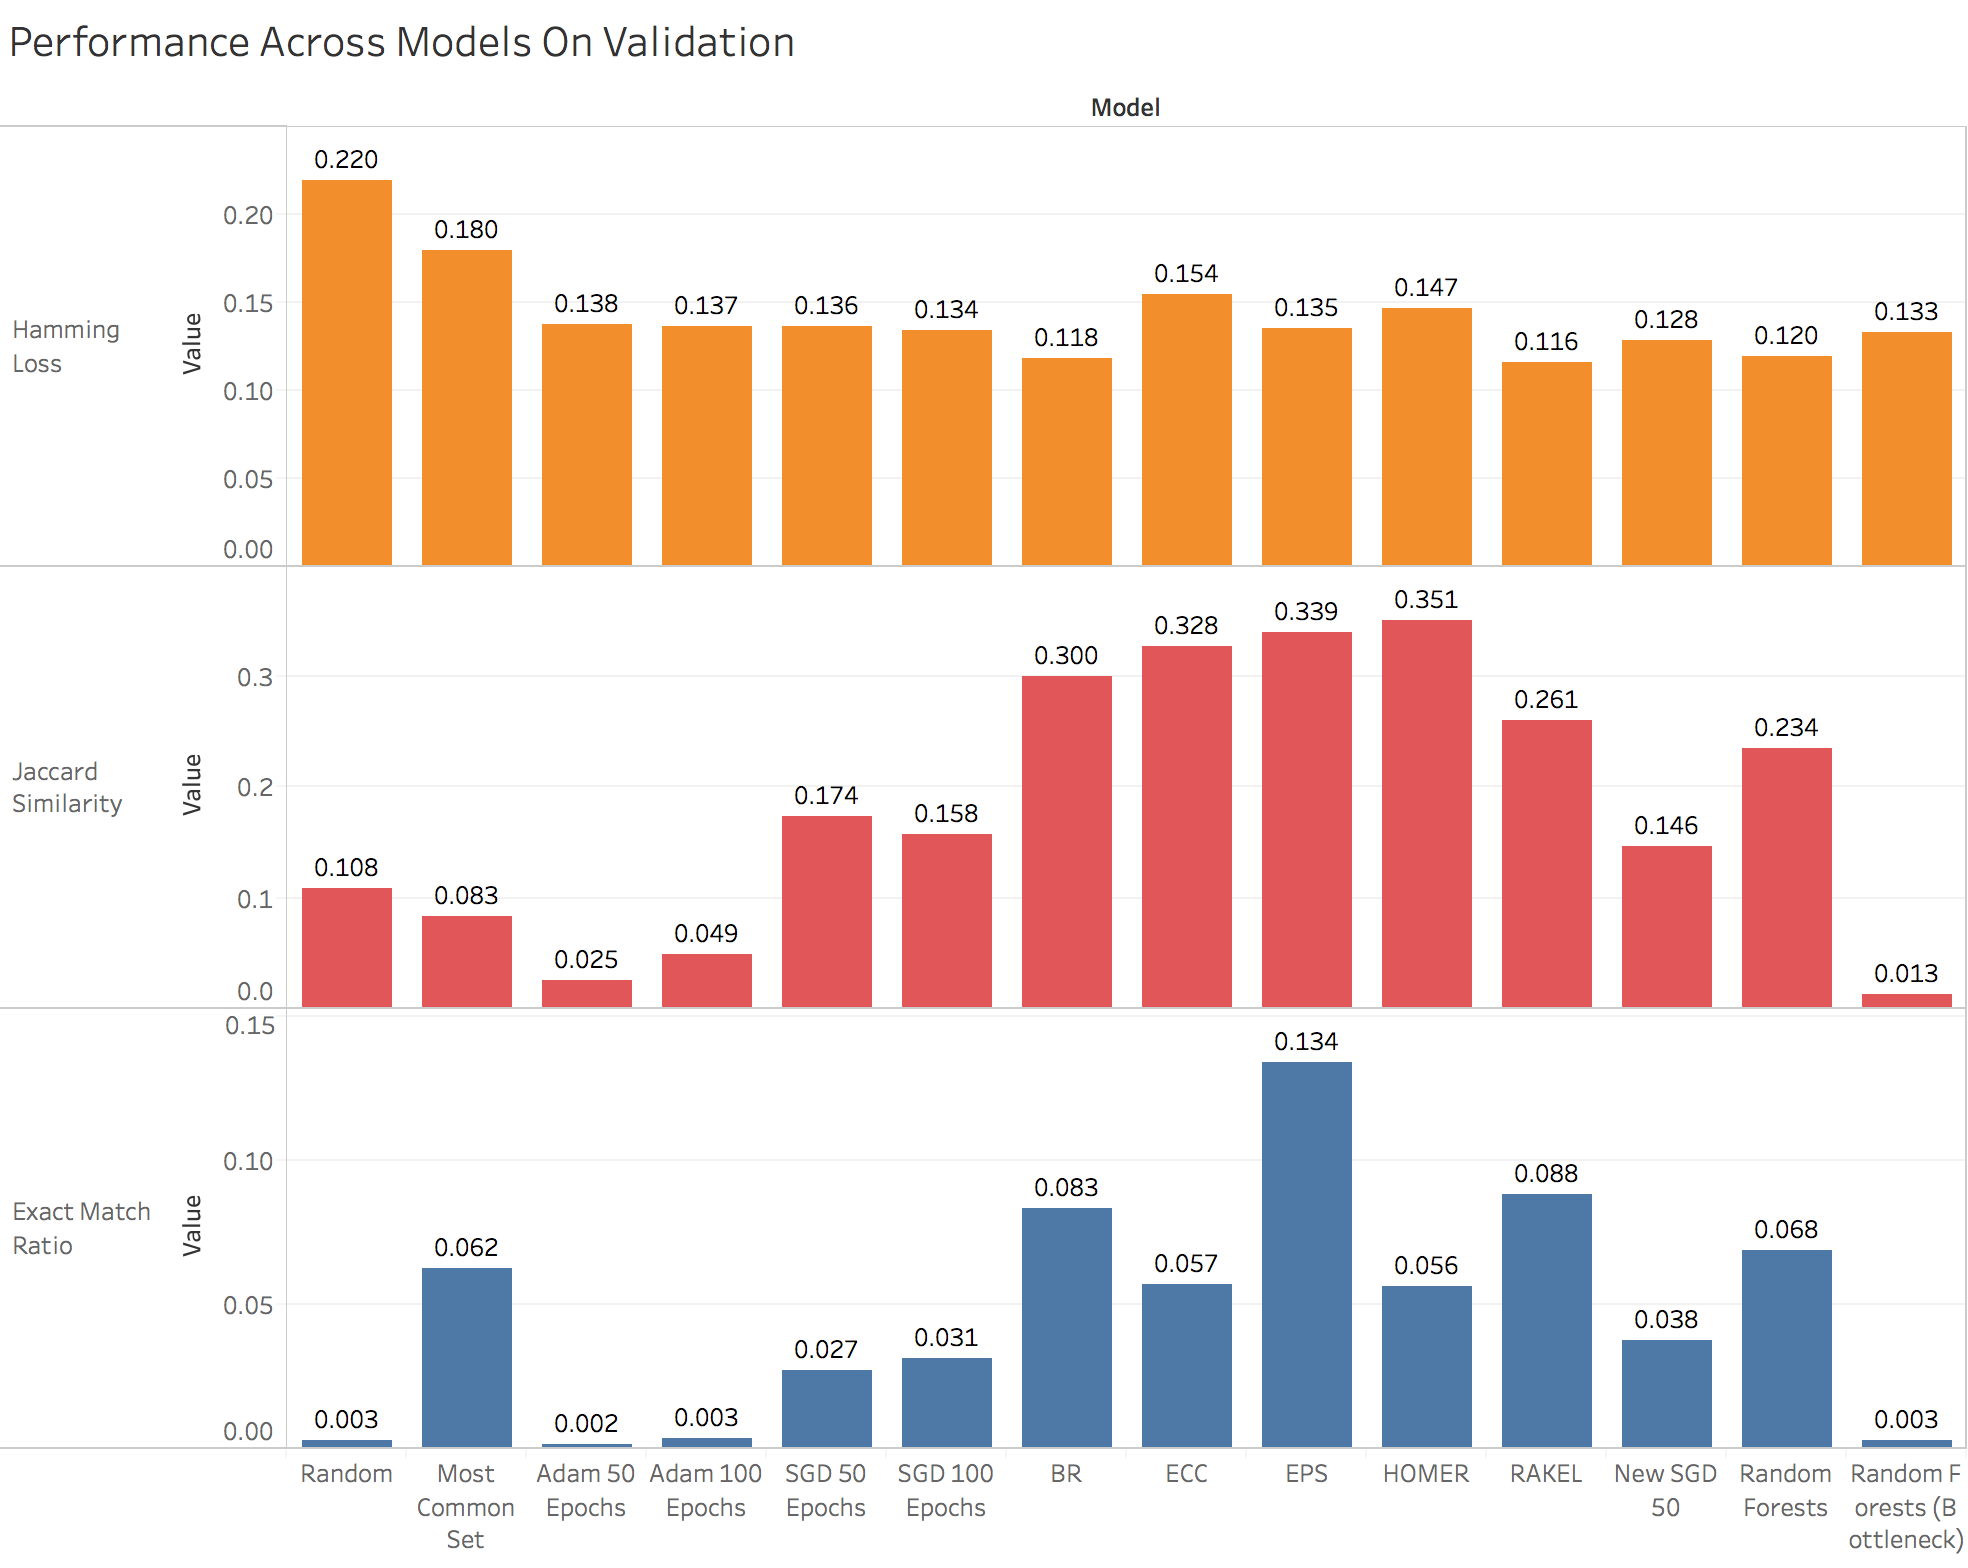
\includegraphics[width=15.5cm]{Models.png}
    \end{center}
    
        \begin{center}
        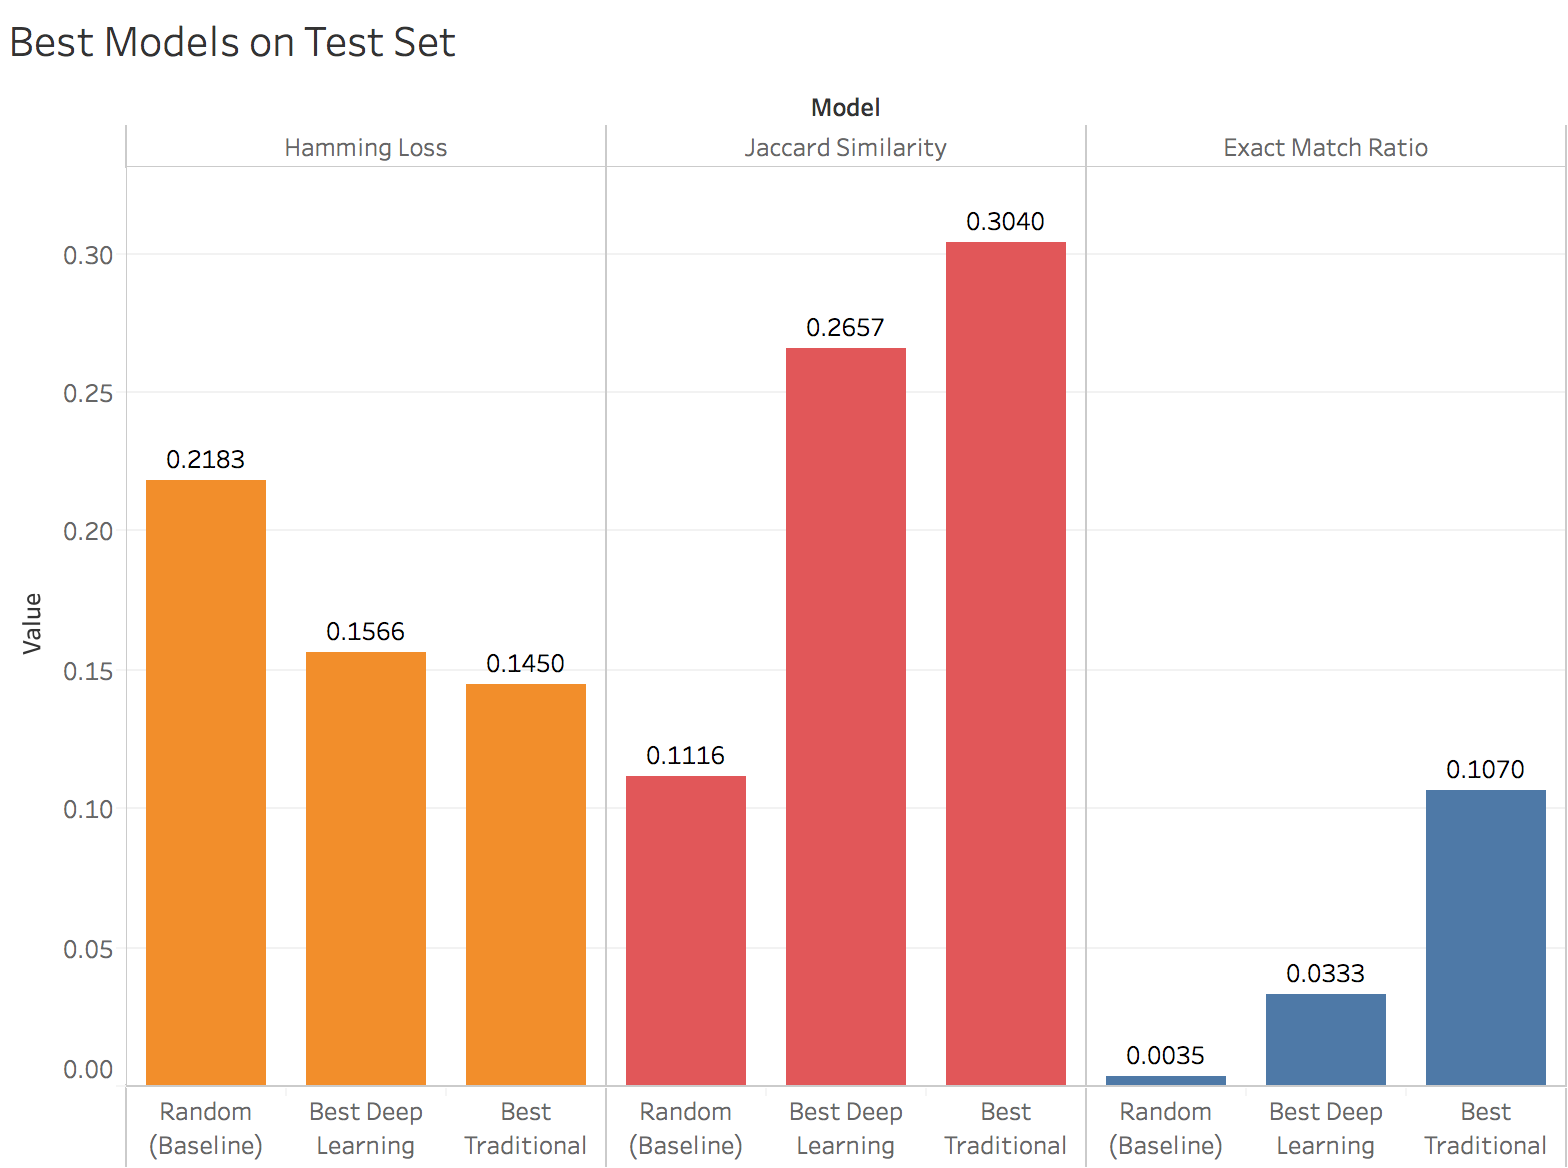
\includegraphics[width=11.5cm]{Test.png}
    \end{center}
    
    \subsection{Evaluation Metrics}
    \indent 
    
    What makes evaluating multilabel classification so difficult is that there is currently no ``standard'' metric for evaluating accuracy. The most common metrics, each with their own pros and cons, are briefly described:
    
        \textbf{Hamming Loss:} Hamming loss is the wrong labels in a prediction divided by the total labels in a prediction. It ignores label dependence. Lower is better.
        
        \textit{Ex.}\\
        \indent True: $(1, 0, 0, 0, 0)$\\
        \indent Pred: $(1, 1, 1, 0, 0)$\\
        \indent Hamming Loss: $2 / 5 = 0.4$
        
        \textbf{Jaccard Similarity:} Jaccard similarity (aka Hamming Score aka Jaccard Coefficient aka Accuracy) is the ratio of the intersection of the true and predicted against the union of the true and predicted. This takes into account label dependence somewhat. Higher is better.
        
        \textit{Ex.}\\
        \indent True: $(A, 0, 0, D, 0)$\\
        \indent Pred: $(A, B, C, 0, 0)$\\
        \indent Jaccard Similarity: $|\{A\}| / |\{A, B, C, D\}| = \frac{1}{4} = 0.25$
        
        \textbf{Exact Match Ratio (aka Subset Accuracy):} This is the proportion of the observations that are perfectly predicted. In this, label dependence is entirely taken into account, in contrast with Hamming Loss. Higher is better.
        
        \textit{Ex.}\\
        \indent True: $(1, 0, 0, 0, 0)$\\
        \indent Pred: $(1, 1, 1, 0, 0)$\\
        \indent Exact Match Ratio: $0 / 1 = 0$
    
    \subsection{Analysis of Results}
    \indent
    
    
    \textbf{Analysis of Results on Validation:}
    For reference, the Most Common Set baseline is the multilabel that appears most frequently in the data (majority multilabel classifier).
    Here we see generally better performance from the traditional methods using the metadata than the naive baseline models and the deep learning models.  This may be explained by the additional information present in the metadata compared to just the posters, as well as the difficulty in tuning deep learning models.
    
    \textbf{Analysis of Results on Test Set:}

    The random baseline predictions were created by randomly selecting genres for each observation in proportion to the average number of genres per movie. The probability that a given genre was selected for a given movie was given by:
    $$P(genre = 1) = \frac{\text{MEAN NUMBER OF GENRES PER MOVIE}}{\text{TOTAL NUMBER OF GENRES}}$$

    The best deep learning model was SGD with 50 epochs, fine-tuned last convolutional layer, and tuned threshold. It performs better than the random baseline model. 
    
    The best traditional model was Ensembles of Pruned Sets. It also produced the best results of any model, particularly with the Exact Match Ratio. This shows that pruning rare sets of genres greatly increases performance, suggesting that rare sets of genres distort the predictive power of other models. 
    
    
    
    % \textbf{Sanity Check for Deep Learning Model}:    
    % As a sanity check to get a more intuitive sense of how our best network performed given that the exact match ratio was relatively low, we also measured its performance on a more relaxed task: accuracy in correctly predicting the most probable genre it outputs for each movie. Specifically, for each movie we took the vector of probabilities for each genre output by the model, took the highest probability as the prediction for that movie's genre and counted it as a correct prediction if that genre was contained in the movie's multilabel. For this relaxed task, our neural network performed well, yielding an accuracy of 53\% on the test set, which assured us that our model was picking up more than just noise. Since this was merely a sanity check as opposed to a formal measure of performance and given that our focus was on the multilabel classification task, we did not conduct this test on our other models.
    


\section{Discussion}    
    \subsection{Interpretation of Deep Learning Results}
    
    \indent 
    
    Obviously, our accuracy measures do have their limitations since they are single number summaries of complex datasets. Therefore, we also evaluated the performance of our final tuned CNN through visualization as well. In particular, we plotted correlation heatmaps of our CNN's genre predictions and also visually inspected the most probable movies for each genre output by our neural net.
        
        \textbf{Genre Correlations Learned}:
        Despite the fact that each of the 20 sigmoids in the final layer of our neural network can output any probability between 0 and 1, they are inherently dependent on one another since they are all part of the same neural network with shared weights. Therefore a natural question to ask would be whether our neural network successfully learned correlations between genres. To address this question we plotted and compared correlation heatmaps for both the CNN's predictions (right figure) and the actual multilabels (left figure) on the validation set:
        
        \begin{center}
            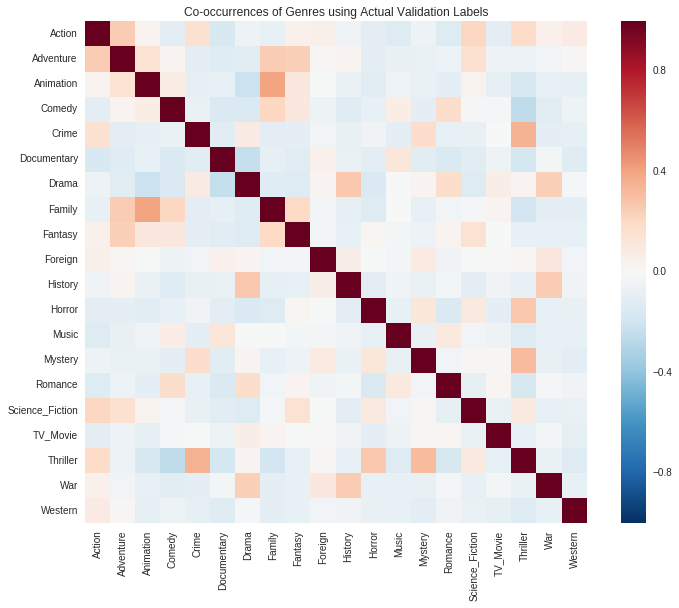
\includegraphics[width=8cm]{heatmap_actual.png}
            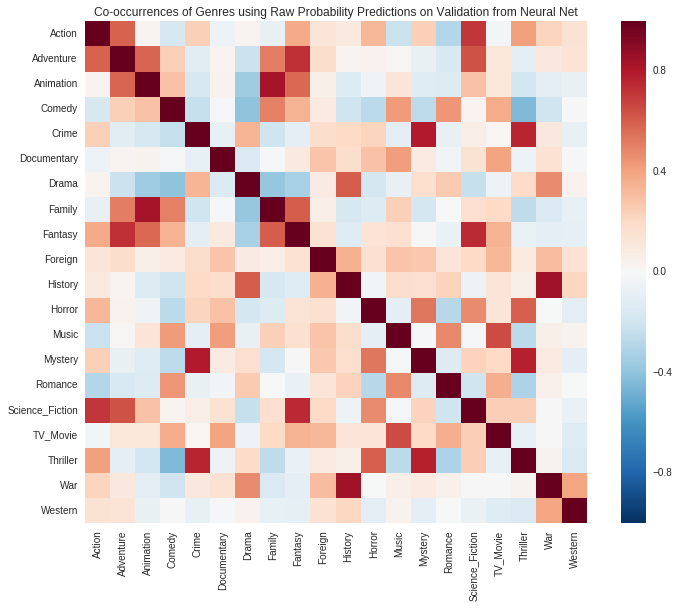
\includegraphics[width=8cm]{heatmap_pred.png}
        \end{center}
        
        We see that many of the correlation structures that exist in the actual multilabels (Action-Adventure, Family-Animation etc.) exist in the predicted multilabels as well.
        
        \textbf{Most Representative Movies per Genre}
        Additionally for each genre, we pulled the top 5 highest probability predictions from the CNN across all movies for that genre to get a sense of the most representative movies for each genre. We see evidence of the CNN perhaps picking up abstract features, such as color schemes and objects. For example, the most representative crime movies tend to be dark and have guns, while animation movies tend to be brightly colored and cartoonish. The least interpretable representative images come from genres like Foreign, which is probably due to a lack of enough training data. The top 3 most representative images for a few select genres are listed below. More detailed interpretations and representative images for all genres can be found in our notebook for Milestone 5. 
        
        \begin{center}
            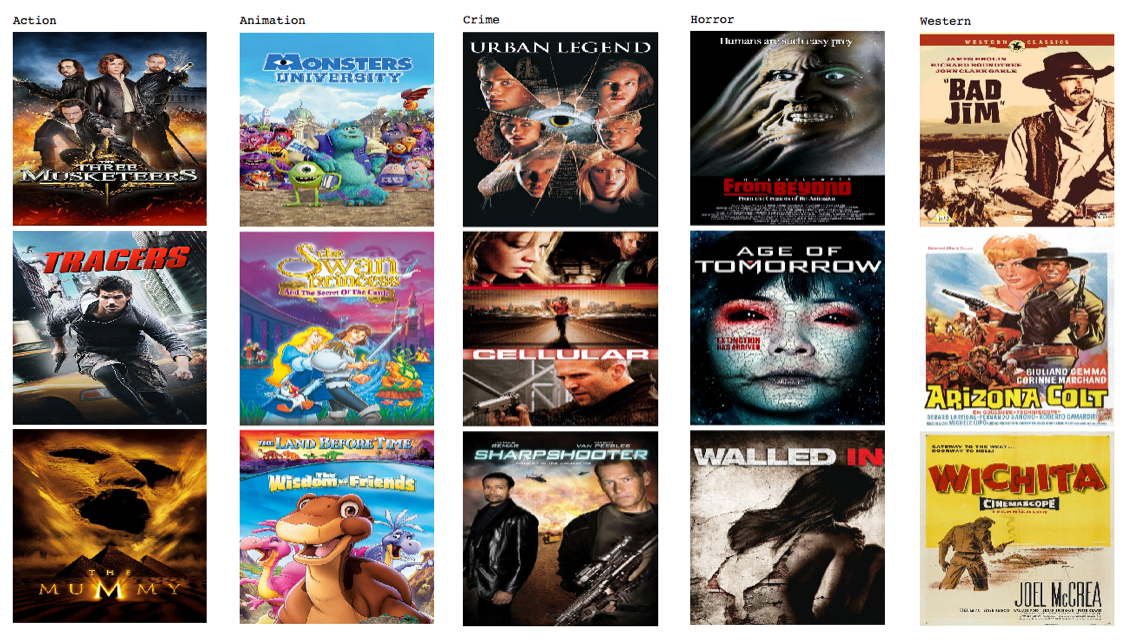
\includegraphics[width=16cm]{mostrepresentative}
        \end{center}
        

        
    \subsection{Further Tuning of Deep Learning Model}
    \indent 
    
    Given the relatively short time frame with which we had to familiarize ourselves with Keras, there obviously was much more tuning and experimentation we could have done. In particular, the greatest drawback was that we were training with binary cross-entropy loss as opposed to a specialized loss function specifically for multilabel classification. For example, the literature lists specialized methods for this very task such as Back-Propagation Multi-Label Learning (BPMLL), which are not built into Keras and we did not have the time to implement from scratch. If we were to continue using binary cross-entropy loss, another avenue of exploration would be experimenting further with modifying the threshold at which we predict a positive instance for each genre. Even with our relatively simple approach of conducting a gridsearch on the training set of which threshold (same one used for all genres) yielded the highest exact match ratio and using that best threshold on the test set, we saw a noticeable boost in performance. Therefore more sophisticated methods of thresholding may yield even better performance.

\section{Conclusion}
    \indent
    
    Two main takeaways from this project were the robustness of traditional methods for multilabel classification and the challenging nature of deep learning. Our best traditional model using metadata outperformed our best deep learning model using movie poster images in every metric we calculated. Nonetheless, judging from visualizations we performed, our deep learning model appears to have successfully learned higher-level visual features of posters for each genre, exceeding our expectations for a model architecture that was not designed specifically for movie genre multilabel classification. How to actually construct such architectures is still a very active area of research, and with our team's limited computational resources and deep learning experience, this task proved difficult. However, given more time, we believe we would have achieved better results by exploring additional ways of customizing our neural net architecture (by unfreezing more layers for instance) and obtaining a larger training set.  
\end{document}

